%!TEX root = batch-course.tex
%-------------------------------------------------
\section{Batch systems}
%-------------------------------------------------
% Related concepts: phases, Z, trajectories, alignment, recipes, operators, manual steps, unfolding, charge reactor

\begin{frame}\frametitle{Batch systems: concepts and unique features}

\begin{itemize}
	\item 	Start point, an end point, and time-based evolution of tags (variables) in between 
	
	\item 	Operate essentially in open-loop i.t.o. critical quality attributes (CQAs).  Basic, low-level feedback. \pause
	
	\item 	Quality measurements made afterwards, usually in a lab
	
			\begin{itemize}
				\item	used to decide batch disposition
				\item	often used to adjust next batch (batch-to-batch control)
			\end{itemize}\pause
			
	\item	Sequenced very accurately
	
	\item	Often have phase-based sequencing

\end{itemize}
\end{frame}

\begin{frame}\frametitle{Batch systems: concepts and unique features}

\begin{itemize}
	
	\item	Nonlinear relationship between variables; those relationships change with time \pause
	
	\item	Poor mechanistic models available (understandable)
	
			\begin{itemize}
				\item	continuous: one or two things happening all the time
				
				\item	batch: series of phases/events and relationships differ between (and within!) phases: very hard to model
				
				\item	complex vapour, liquid and solid phase interactions in a batch
			\end{itemize} \pause
			
	\item 	Past history within a batch affects the future
	
			\begin{itemize}
				\item	initial conditions: affect trajectories and CQAs
				
				\item	trajectory changes from operator affect CQAs
				
				\item	actions taken can affect some period or all of batch, or,
				
				\item	even have no effect - relevant when monitoring a batch
			\end{itemize}
			
	
	\item	\emph{Discussion of your experience on these topics.}
\end{itemize}
\end{frame}

\begin{frame}\frametitle{Batch systems: terminology for these notes}

\begin{description} 
	
	\item[ \( N \): number of batches] 
	
		\begin{itemize}
			\item	literature uses \( I \)
		\end{itemize}
		
	\item[\( K \): number of tags] 
	
		\begin{itemize}
			\item	 literature uses \( J \)
		\end{itemize}
	
	\item[\( J \): number of time steps, ] 
	
		\begin{itemize}
			\item	 literature uses \( K \)
		\end{itemize}
\end{description}

We aim for consistency with general latent variable methods: \( N \times K \times J \)

\begin{center}
	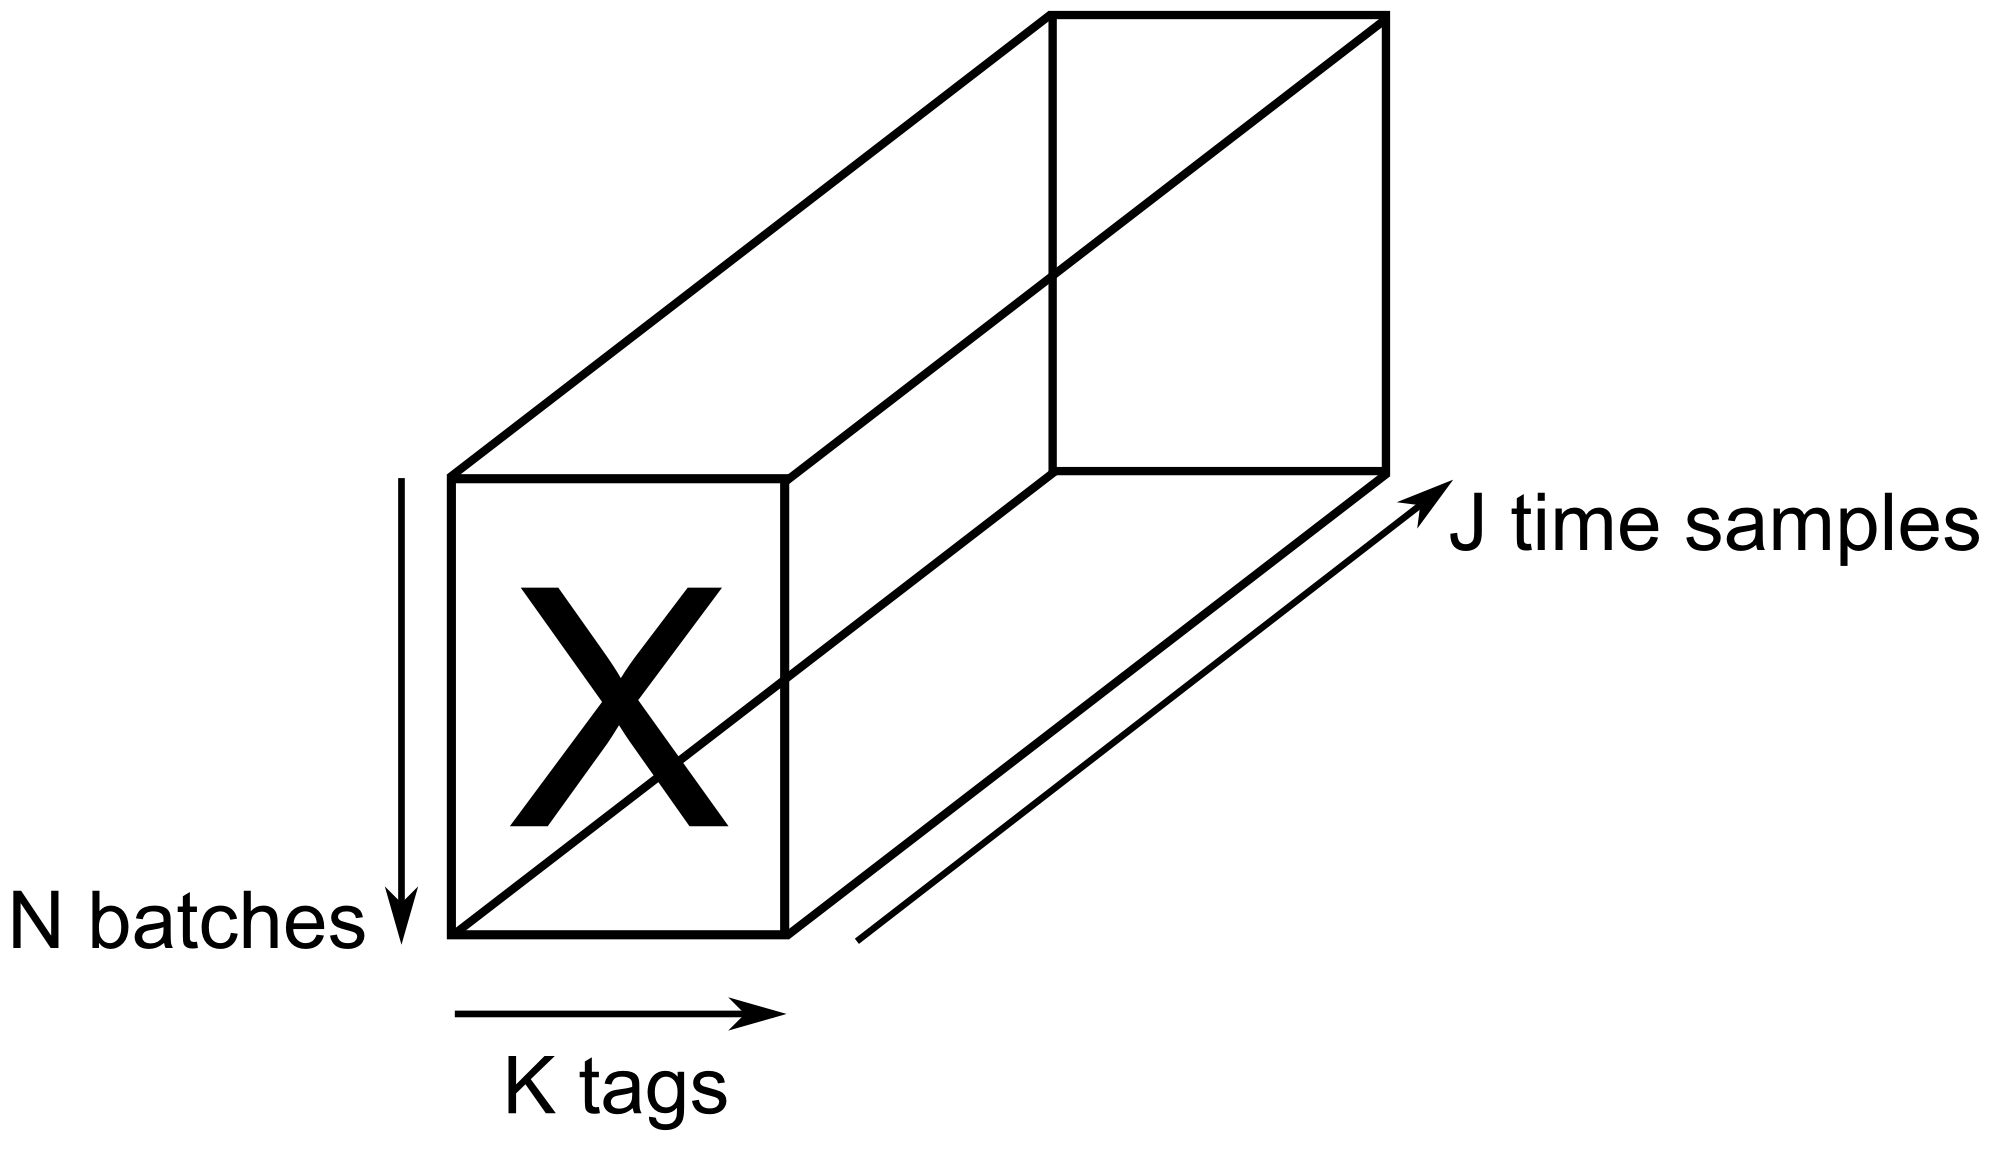
\includegraphics[width=7.2cm]{images/batch-data-cube.png}
\end{center}

\end{frame}

\begin{frame}\frametitle{Batch systems: data representation}

When retrieving batch data from computerized systems:
\begin{enumerate}
	\item	One batch per sheet in a spreadsheet, with batch ID
			
			
\includegraphics[scale=0.75]{images/batches-in-spreadsheets.png}
	
	\item	One batch per CSV file
\end{enumerate}
\end{frame}

\begin{frame}\frametitle{Batch systems: data representation}

\begin{enumerate}
	\setcounter{enumi}{2}
	\item	Stacked batches of \textbf{equal duration} in a single file

			\begin{center}
				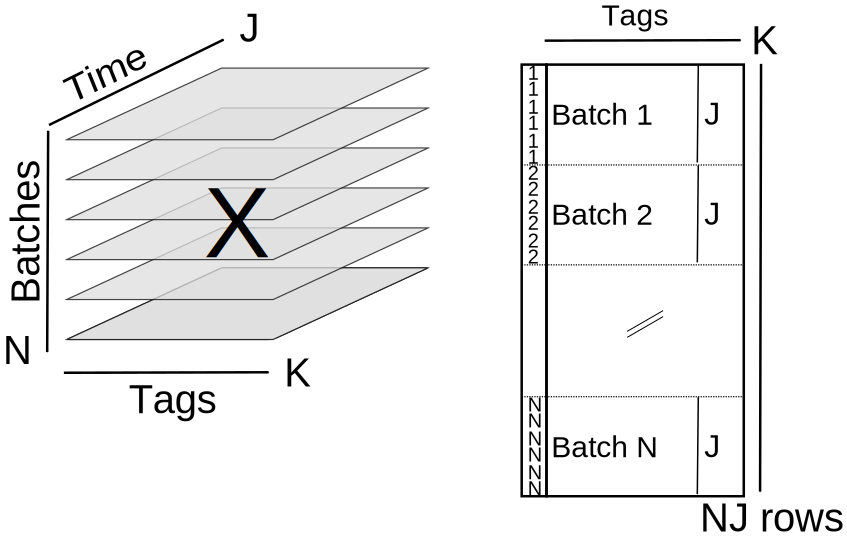
\includegraphics[width=0.9\textwidth]{images/batch-data-layers-into-page-and-unfolded-aligned}
			\end{center}
					
\end{enumerate}
The extra batch ID column is optional.  Some batch software require the data input this way.
\end{frame}

\begin{frame}\frametitle{Batch systems: data representation}

\begin{enumerate}
	\setcounter{enumi}{3}
	\item	Stacked, \textbf{but unaligned} batches, in a single file (common)
			
			\begin{columns}
				\column{.3\textwidth}
					\begin{itemize}
						\item	must also include a batch ID column

						\item	phased recipes: append a ``phase ID'' column within each batch (not shown)
					\end{itemize}
					
				\column{0.7\textwidth}
				
					\begin{center}
						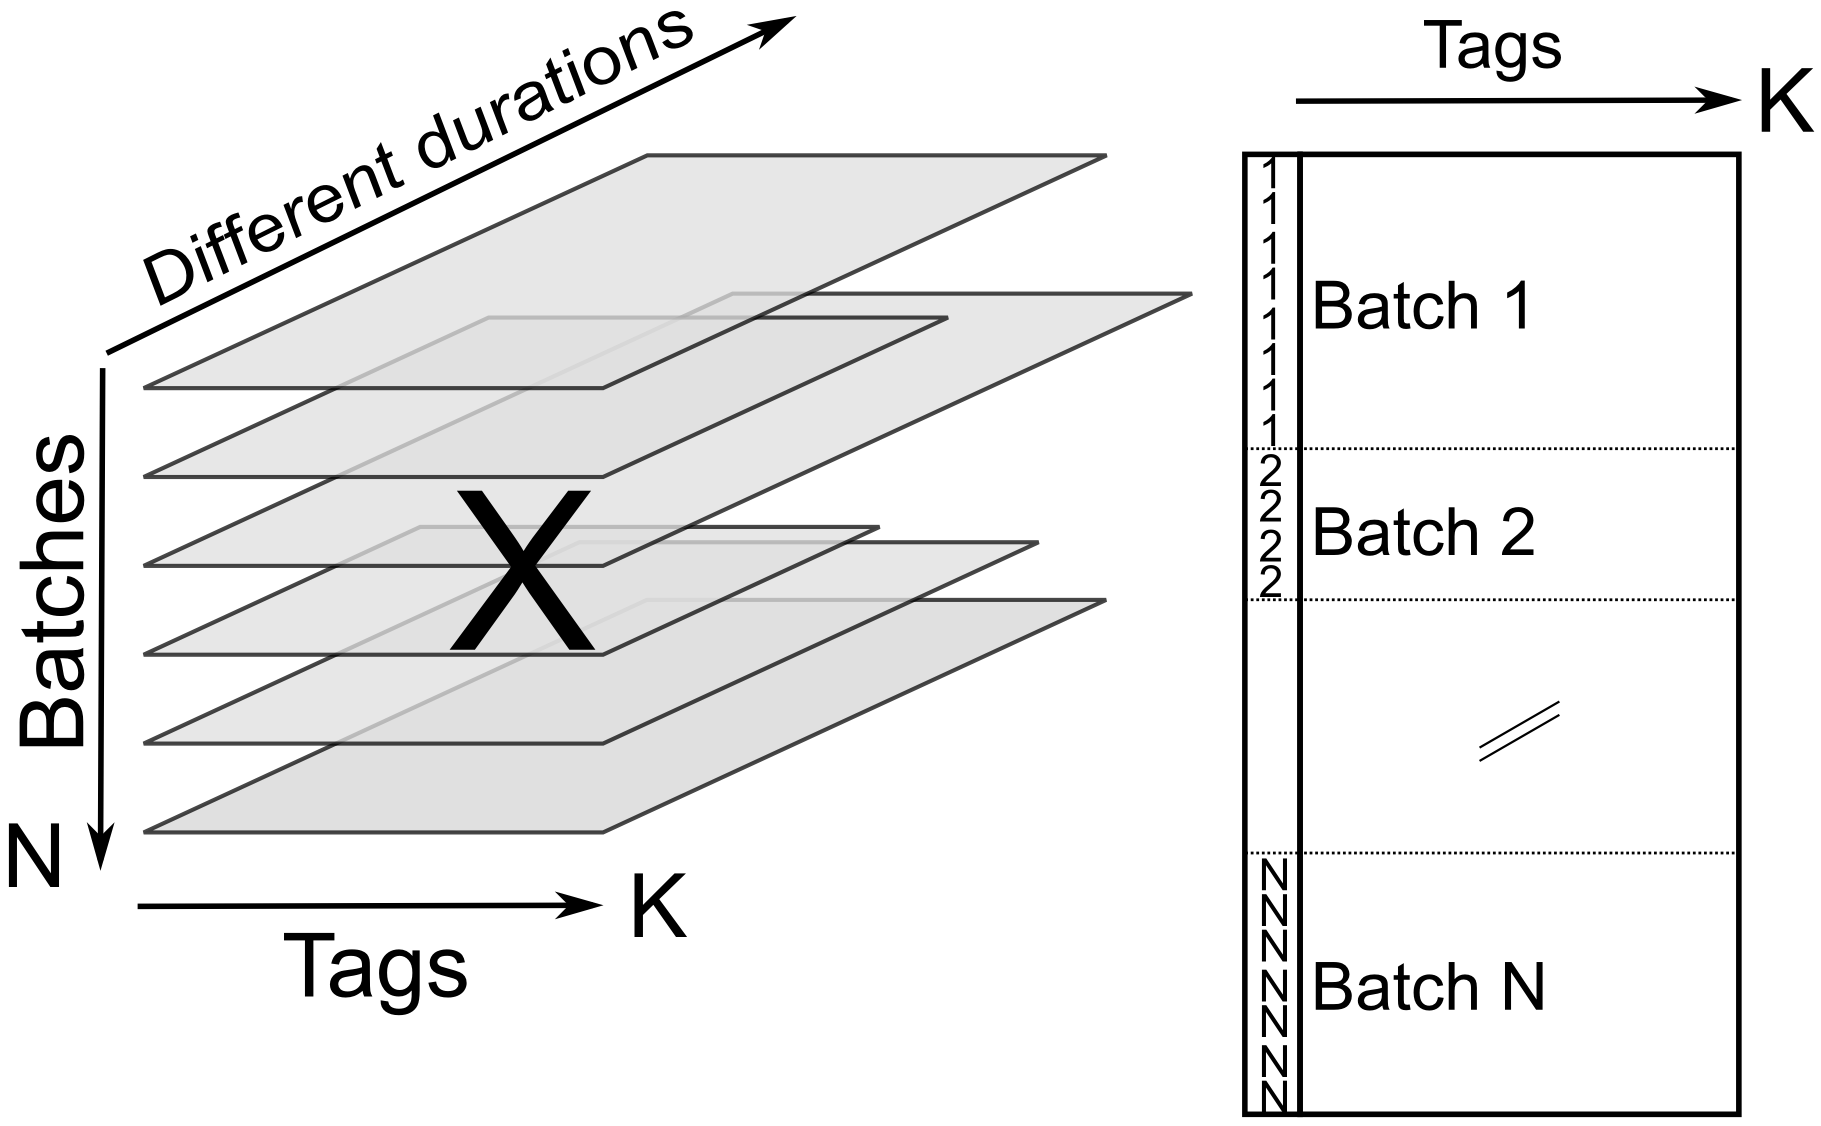
\includegraphics[width=\textwidth]{images/batch-data-layers-into-page-and-unfolded.png}
					\end{center}
					
			\end{columns}
\end{enumerate}
MATLAB can handle all the formats shown above.
\end{frame}

\begin{frame}\frametitle{Batch systems: data representation}
	
	\begin{itemize}
		\item	It is very common that the time-dimension, \( J \), is unequal	
		
		\item	We deal later with alignment: equalizing the time-dimension for all batches
	\end{itemize}
\end{frame}

\begin{frame}\frametitle{Batch systems: visualize the trajectory data}
	
	\begin{columns}
		\column{.40\textwidth}
			{\color{myOrange}{\textbf{Unaligned data}}}
 			\vfill
			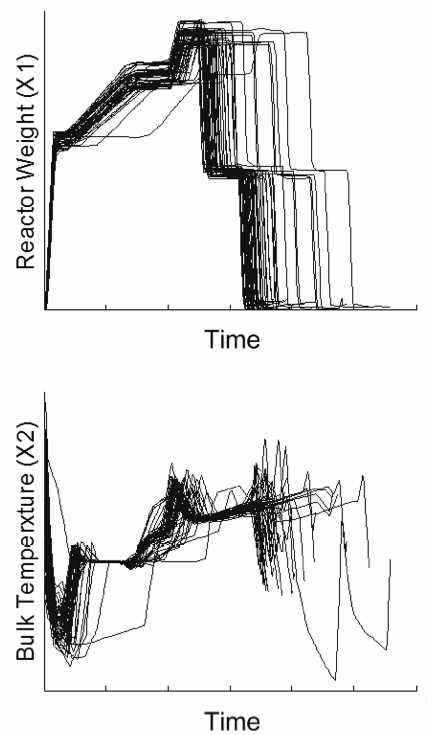
\includegraphics[height=0.8\textheight]{images/unaligned-trajectories-many-batches.png}
			% From Cecilia Rodrigues thesis, used with permission (see gmail email in February 2011)
		
		\column{.60\textwidth}
			{\color{myOrange}{\textbf{Aligned data}}}
			\vfill
			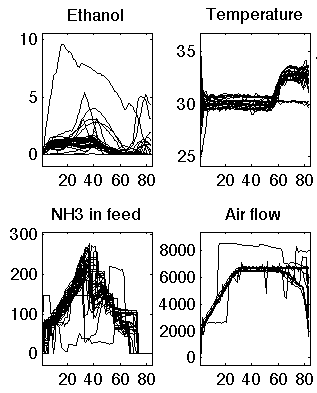
\includegraphics[height=0.8\textheight]{images/aligned-trajectories-many-batches-yeast.png}
			% Using rev 85:95b49ee15280 			
			% data = load('/Users/kevindunn/ConnectMV/Courses/Batch/datasets/yeast/yeast-data.mat');
			% b.tagNames = {'Ethanol', 'Temperature', 'Molasses', 'NH3 in feed', ...
			%               'Air flow', 'Tank level', 'pH'};
			% b.batchnames = {'rB','rC','rI','rM','rN','rQ','rR','rT','rV','rX','rZ', ...
			%                'ra','rb_1','rc_1','rd','re','rf','rg','rh','ri_1','nA', ...
			%                'tD','nG','nH','tJ','nL','nO','tP','nU','nY','rj','rk','rl'};
			% b.nBatches = 33;
			% batch_X = block(data.X, 'X', 'batch', 'tagNames', b.tagNames, 'nBatches', b.nBatches);
			% plot(batch_X, 'raw', 2, 3) % but used a limited set
	\end{columns}

\end{frame}

